%!TEX root = ../main.tex

\subsection[Calibration using \texorpdfstring{$\BdToDsD$}{Bd2DsD}]{Calibration using \texorpdfstring{$\BdToDsD$}{Bd2DsD}}
\label{sec:dataanalysis:taggingcalibration:dsdcalibration}

The decay of \Bd mesons via the decay mode \BdToDsD proceeds flavour specific
as the charge of the \Dsp meson unambiguously determines the flavour of the
decaying \Bd meson. When reconstructing the \Dsp meson via \DspToKKpi and the
\Dp meson via \DpToKpipi, a very similar selection to the one for \BdToDD
(described in \cref{sec:b02dd:selection}) can be applied. The only differences
are that the invariant $m_{\KKpi}$ mass is required to lie within
\SI{\pm25}{\MeVcc} of the known \Dsp mass~\cite{PDG2014} and that the vetoes
against misidentified backgrounds are not applied. A maximum likelihood fit to
the invariant $m_{\DsD}$ mass distribution is performed to statistically
subtract the remaining background via the \sPlot technique. Apart from the
\BdToDsD component, which is parametrised by the sum of two Crystal Ball
functions (common mean but different widths, and tail parameters taken from
MC), the fit model includes components for \BsToDsD decays and for
combinatorial background. The total \BdToDsD yield is found to be
$\num{16736\pm134}$ at a quite low background level as can be seen in
\cref{fig:dataanalysis:taggingcalibration:dsdcalibration:mass}.

\begin{figure}[htb]
\centering
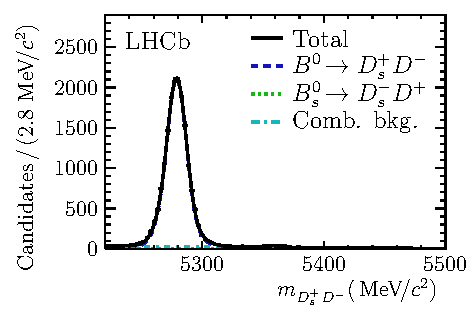
\includegraphics[width=0.48\textwidth]{05-DataAnalysis/tikz/pdf/DsD_MassFit.pdf}
% \includegraphics[width=0.48\textwidth]{tikz/pdf/FigApp_DsD_MassFit_log.pdf}
\caption{Masses of \BdToDsD candidates and projected PDFs.}
%, shown with a linear scale on the vertical axis (left) and a logarithmic scale (right).
\label{fig:dataanalysis:taggingcalibration:dsdcalibration:mass}
\end{figure}

The $\Bd$--$\Bzb$ mixing prevents to infer the flavour of the \Bd meson at
production. Therefore, a mixing analysis is performed to determine the true
mistag probability $\omega$ from the amplitude of the mixing asymmetry
\begin{equation}
\mathcal{A}^{\text{mix}}_{\text{meas}} (t) \equiv \frac{N_{\text{unmixed}}(t) - N_{\text{mixed}}(t)}{N_{\text{unmixed}}(t) + N_{\text{mixed}}(t)}
 =(1-2\omega) \cos(\dmd\,t) \,,
\label{eq:dataanalysis:taggingcalibration:dsdcalibration:asymmetry}
\end{equation}
where $N_{\text{unmixed}}$ is the number of \BdToDsD decays with a final state
that does correspond to the flavour tag, and $N_{\text{mixed}}$ the number
with a final state that does not. Other experimentally induced effects are
corrected for, like the detection asymmetry $\mathcal{A}_{\mathrm{det}}$, the
production asymmetry $\AP$ and the flavour-specific asymmetry
$a_{\mathrm{sl}}^d$. With unbinned maximum likelihood fits to the decay time
and tag distributions the results listed in
\cref{tab:dataanalysis:taggingcalibration:dsdcalibration} are determined, one
fit for the sample with a non-zero tag of the OS tagging combination and one
for the sample with a non-zero tag of the SS tagging combination. This means
that some candidates are used for both calibrations. The systematic
uncertainties are dominated by the background subtraction and the calibration
method.

\begin{table}[htb]
\caption{Flavour-tagging calibration parameters from \BdToDsD. The first
uncertainty is statistical and the second accounts for systematic
uncertainties.}
\label{tab:dataanalysis:taggingcalibration:dsdcalibration}
\centering
\begin{tabular}{lr@{$\,\pm\,$}l@{$\,\pm\,$}lr@{$\,\pm\,$}l@{$\,\pm\,$}l}
  \toprule
  Parameter             & \multicolumn{3}{c}{OS} & \multicolumn{3}{c}{SS} \\
  \midrule
  $p_{1}$               & 1.07  & 0.07  & 0.01  & 0.84  & 0.09  & 0.01  \\
  $p_{0}$               & 0.369 & 0.008 & 0.010 & 0.430 & 0.006 & 0.009 \\
  $\langle \eta\rangle$ & \multicolumn{3}{c}{0.3627} & \multicolumn{3}{c}{0.4282} \\
  $\Delta p_{1}$        & 0.03  & 0.11  & 0.03  & 0.07   & 0.13  & 0.05  \\
  $\Delta p_{0}$        & 0.009 & 0.012 & 0.001 & -0.007 & 0.009 & 0.001 \\
  \bottomrule
\end{tabular}
\end{table}

The raw mixing asymmetries in
\cref{fig:dataanalysis:taggingcalibration:dsdcalibration:rawasymmetries}
represent graphically that the OS tagging combination on average provides
better mistag estimates but has a lower tagging efficiency than the SS tagging
combination. This can be derived from the larger amplitude and the larger
error bars.

\begin{figure}[htb]
\centering
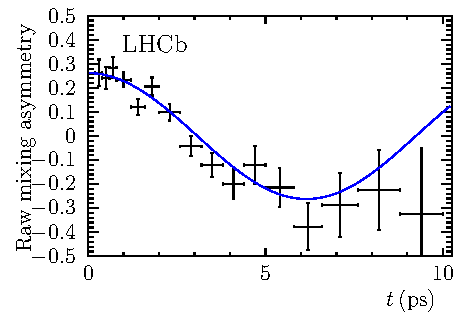
\includegraphics[width=0.48\textwidth]{05-DataAnalysis/tikz/pdf/DsD_MixingAsym_OSComb.pdf}
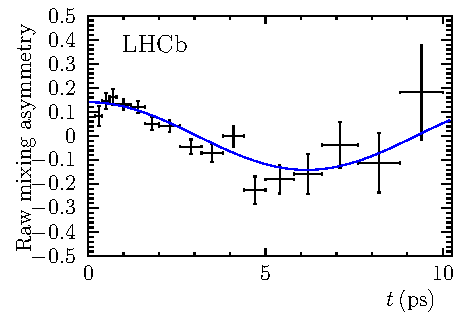
\includegraphics[width=0.48\textwidth]{05-DataAnalysis/tikz/pdf/DsD_MixingAsym_SSComb.pdf}
\caption{Raw mixing asymmetry as a function of the \Bd decay time for events
tagged by (left) the OS and (right) the SS tagging combination. The solid line
represents the PDF projection.}
\label{fig:dataanalysis:taggingcalibration:dsdcalibration:rawasymmetries}
\end{figure}

Thanks to the improved flavour-tagging algorithms and the kinematic properties
of the selected \BdToDD decays, which for example have on average a higher
\pT, an effective tagging efficiency of $\etag D^2= \SI{8.1\pm0.6}{\percent}$
is achieved. This splits into a tagging power of \SI{1.02\pm0.09}{\percent}
from events that are tagged only by OS taggers, \SI{1.36\pm0.19}{\percent}
from events tagged only by SS taggers, and \SI{5.7\pm0.5}{\percent} from
events tagged by tagging algorithms of both sides. To date it's the highest
effective tagging efficiency in tagged $\CP$ violation measurements at \lhcb.

The flavour-tagging calibration using \BdToDsD decays has been provided by
collaborators from Milano.

% The tagging efficiency is \etag = \SI{87.6\pm0.8}{\percent} and the effective
% dilution $D = 1 - 2\mistag = \SI{30.3\pm1.1}{\percent}$.
